\documentclass[10pt]{beamer}
\usefonttheme{professionalfonts,serif}
\def\newblock{\hskip .11em plus .33em minus .07em}
\usepackage[numbers,sort]{natbib}
\renewcommand{\rmdefault}{psbx}
\usepackage[utf8]{inputenc}
\usepackage[T1]{fontenc}
\usepackage{textcomp}
\usepackage{eulervm}

\usetheme{default}           % tips from David Blei
\useinnertheme{circles}
\useoutertheme{infolines}
\setbeamertemplate{headline}{}
\setbeamertemplate{navigation symbols}{}
\setbeamerfont{itemize/enumerate subbody}{size=\normalsize}
\setbeamerfont{itemize/enumerate subsubbody}{size=\normalsize}
\usecolortheme{seahorse}
\setbeamersize{text margin left=2mm,text margin right=2mm}

\graphicspath{{../../figures/}}

\definecolor{mypine}{rgb}{0.05,0.45,0.05}
\definecolor{mycyan}{rgb}{0.0,0.9,0.9}
\newcommand{\Red}{\textcolor{red}}
\newcommand{\Blue}{\textcolor{blue}}
\newcommand{\Green}{\textcolor{mypine}}
\newcommand{\PineGreen}{\textcolor{mypine}}
\newcommand{\Magenta}{\textcolor{magenta}}
\newcommand{\Cyan}{\textcolor{mycyan}}

\newcommand{\N}{\mathcal{N}}
\newcommand{\R}{\mathbb{R}}
\newcommand{\T}{{\scriptsize^{\top}}}
\newcommand{\D}{\mathcal{D}}
\newcommand{\F}{\mathcal{F}}
\newcommand{\E}{\mathbb{E}}
\newcommand{\V}{\mathbb{V}}
\newcommand{\M}{\mathcal{M}}
\newcommand{\KL}{\mathcal{KL}}
\newcommand{\cut}[1]{}
\newcommand{\trace}{\operatorname{trace}}

\newcommand{\bmu}{{\boldsymbol{\mu}}}
\newcommand{\btheta}{\boldsymbol{\theta}}
\newcommand{\bepsilon}{\boldsymbol{\epsilon}}
\newcommand{\balpha}{\boldsymbol{\alpha}}
\newcommand{\bbeta}{\boldsymbol{\beta}}
\newcommand{\bphi}{\boldsymbol{\phi}}
\newcommand{\bPhi}{\boldsymbol{\Phi}}
\newcommand{\bSigma}{\boldsymbol{\Sigma}}
\newcommand{\bpi}{\boldsymbol{\pi}}
\newcommand{\blambda}{\boldsymbol{\lambda}}

\newcommand{\argmax}{\operatorname{argmax}}
\newcommand{\argmin}{\operatorname{argmin}}
\newcommand{\ci}{{\bot\negthickspace\negthickspace\bot}} % conditional indep.
\newcommand{\neigh}{\operatorname{ne}}
\newcommand{\vectr}[2]{  \left[ \!\!\begin{array}{c} #1 \\
      #2 \end{array} \!\!\right]}
\newcommand{\deff}{\stackrel{\mathrm{def}}{=}}
\newcommand{\deldel}[2]{\frac{\partial #1}{\partial #2}}

\newcommand{\maketilde}{\raisebox{0.4ex}{\tiny $\sim$}}
\newcommand{\bfa}{\mathbf a}
\newcommand{\bfb}{\mathbf b}
\newcommand{\bfe}{\mathbf e}
\newcommand{\bff}{\mathbf f}
\newcommand{\bfk}{\mathbf k}
\newcommand{\bfm}{\mathbf m}
\newcommand{\bfn}{\mathbf n}
\newcommand{\bfp}{\mathbf{p}}
\newcommand{\bfs}{\mathbf s}
\newcommand{\bfu}{\mathbf u}
\newcommand{\bfx}{\mathbf x}
\newcommand{\bfy}{\mathbf y}
\newcommand{\bft}{\mathbf t}
\newcommand{\bfv}{\mathbf v}
\newcommand{\bfw}{\mathbf w}
\newcommand{\bfA}{\mathbf A}
\newcommand{\bfI}{\mathbf I}
\newcommand{\bfK}{\mathbf K}


\title{Factor Graphs and message passing}
\author{Carl Edward Rasmussen}
\date{October 28th, 2016}

\begin{document}


\begin{frame}
\titlepage
\end{frame}


\begin{frame}
\frametitle{Key concepts}

\begin{itemize}
\item Factor graphs are a class of graphical model
\item A factor graph represents the product structure of a function,
  and contains factor nodes and variable nodes 
\item We can compute marginals and conditionals efficiently by passing
  messages on the factor graph, this is called the sum-product
  algorithm (a.k.a.\  belief propagation or factor-graph propagation)
\item We can apply this to the True Skill graph
\item But certain messages need to be approximated
\item One approximation method based on moment matching is
  called Expectation Propagation (EP)
\end{itemize}

\end{frame}


\begin{frame}
\frametitle{Factor Graphs}

Factor graphs are a type of \emph{\Blue{probabilistic graphical
model}} (others are directed graphs, a.k.a.\ Bayesian networks,
and undirected graphs, a.k.a.\ Markov networks).\\[1ex]

Factor graphs allow to represent the product structure of a
function.\\[1ex]

Example: consider the factorising probability distribution:
\[
p(v, w, x, y, z)\;=\;f_1(v, w)f_2(w, x)f_3(x, y)f_4(x, z)
\]

A factor graph is a bipartite graph with two types of nodes:
\begin{itemize}
\item Factor node: $\blacksquare$ \;\;\;\; Variable node: $\bigcirc$
\item Edges represent the dependency of factors on variables.
\end{itemize}

\centerline{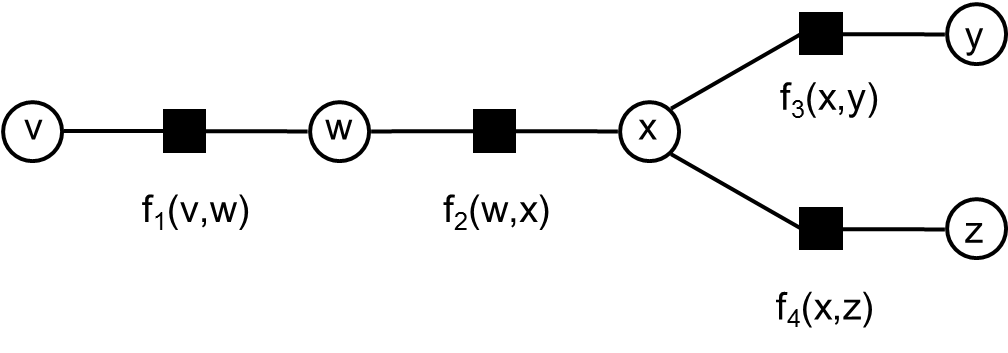
\includegraphics[width=0.6\textwidth]{ExampleFactorGraph1}}

\end{frame}

\begin{frame}
\frametitle{Factor Graphs}

\[
p(v, w, x, y, z)\;=\;f_1(v, w)f_2(w, x)f_3(x, y)f_4(x, z)
\]

\centerline{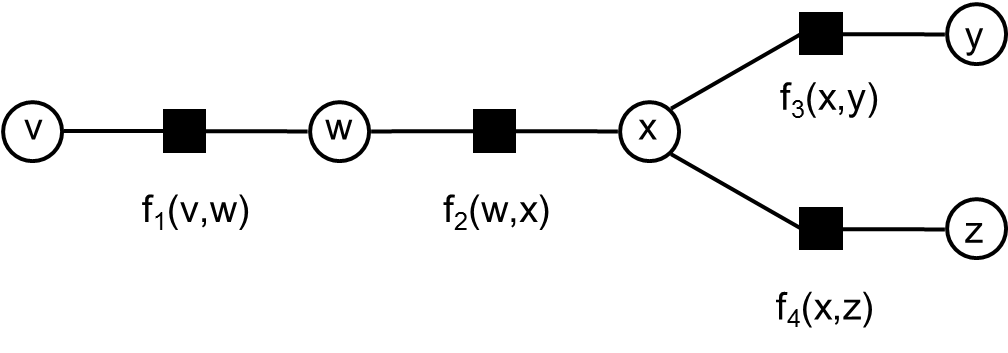
\includegraphics[width=0.6\textwidth]{ExampleFactorGraph1}}

\begin{itemize}
\item What are the marginal distributions of the individual variables?
\item What is $p(w)$?
\item How do we compute conditional distributions, e.g.\ $p(w|y)$?
\end{itemize}

For now, we will focus on \emph{tree-structured} factor graphs.

\end{frame}


\begin{frame}
\frametitle{Factor trees: separation (1)}

\centerline{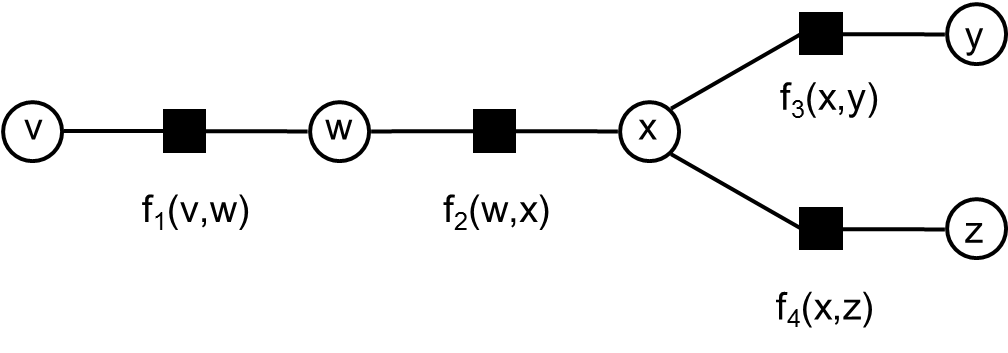
\includegraphics[width=0.6\textwidth]{ExampleFactorGraph1}
}
\[
p(w) = \sum_v\sum_x\sum_y\sum_z f_1(v,w)f_2(w,x)f_3(x,y)f_4(x,z)
\]
\begin{itemize}
\item If $w$, $v$, $x$, $y$ and $z$ take $K$ values each, we have $\approx 3K^4$ 
products and $\approx K^4$ sums, for each value of $w$, i.e.\ total ${\cal O}(K^5)$.
\item Multiplication is distributive: $ca + cb = c(a+b)$.\\ 
The right hand side is more efficient!
\end{itemize}

\hfill

\end{frame}


\begin{frame}
\frametitle{Factor trees: separation (2)}

\centerline{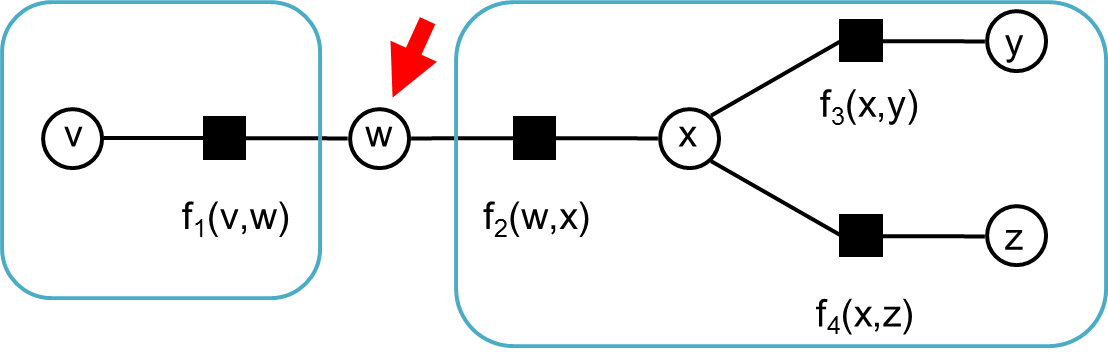
\includegraphics[width=0.67\textwidth]{ExampleFactorGraph2}
}
\begin{eqnarray*}
p(w) &=& \sum_v\sum_x\sum_y\sum_z f_1(v,w)f_2(w,x)f_3(x,y)f_4(x,z) \\
& = & \Big[\!\sum_v f_1(v,w)\!\Big] \cdot
\Big[\!\sum_x\sum_y\sum_z f_2(w,x)f_3(x,y)f_4(x,z)\!\Big]
\end{eqnarray*}
\begin{itemize}
\item In a tree, each node separates the graph into disjoint parts.
\item Grouping terms, we go from sums of products to
  products of sums. 
\item The complexity is now ${\cal O}(K^4)$.
\end{itemize}

% \hfill

\end{frame}

\begin{frame}
\frametitle{Factor trees: separation (3)}

\centerline{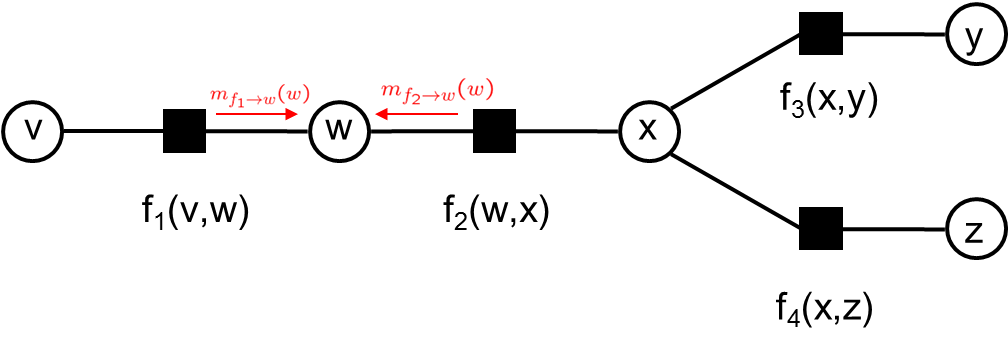
\includegraphics[width=0.7\textwidth]{ExampleFactorGraph3}
}
\[
p(w) = \underbrace{\Big[\!\sum_v f_1(v,w)\!\Big]}_{\Red{m_{f_1\rightarrow w}(w)}}
\cdot
\underbrace{\Big[\!\sum_x\sum_y\sum_z f_2(w,x)f_3(x,y)f_4(x,z)\!\Big]}_{
\Red{m_{f_2\rightarrow w}(w)}}
\]
\begin{itemize}
\item Sums of products becomes products of sums of all messages from
neighbouring factors to variable.
\end{itemize}

\hfill

\end{frame}


\begin{frame}
\frametitle{Messages: from factors to variables (1)}

\centerline{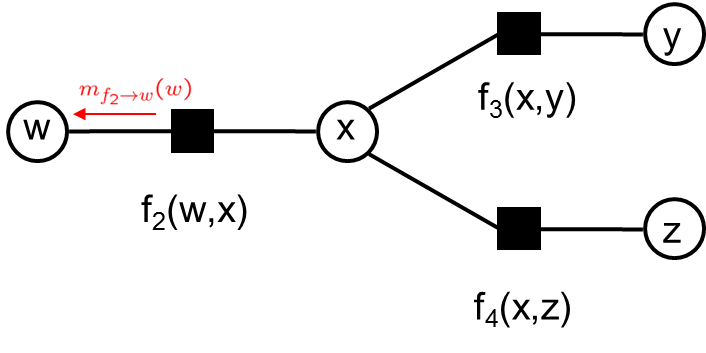
\includegraphics[width=0.45\textwidth]{ExampleMessages1}
}
\[
\Red{m_{f_2\rightarrow w}(w)} = \sum_x\sum_y\sum_z f_2(w,x)f_3(x,y)f_4(x,z)
\]

\phantom{.}
\hfill
\phantom{.}

\end{frame}


\begin{frame}
\frametitle{Messages: from factors to variables (2)}

\centerline{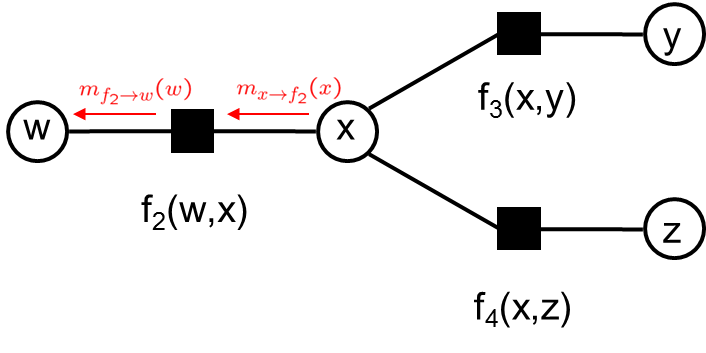
\includegraphics[width=0.45\textwidth]{ExampleMessages2}
}
\begin{eqnarray*}
\Red{m_{f_2\rightarrow w}(w)} &=& \sum_x\sum_y\sum_z
f_2(w,x)f_3(x,y)f_4(x,z) \\
&=& 
\sum_x f_2(w,x) \cdot
\underbrace{\Big[\!\sum_y\sum_z f_3(x,y)f_4(x,z)\!\Big]}_{
\Red{m_{x\rightarrow f_2}(x)}}
\end{eqnarray*}

\begin{itemize}
\item Factors only need to sum out all their local variables.
\end{itemize}

\hfill

\end{frame}


\begin{frame}
\frametitle{Messages: from variables to factors (1)}

\centerline{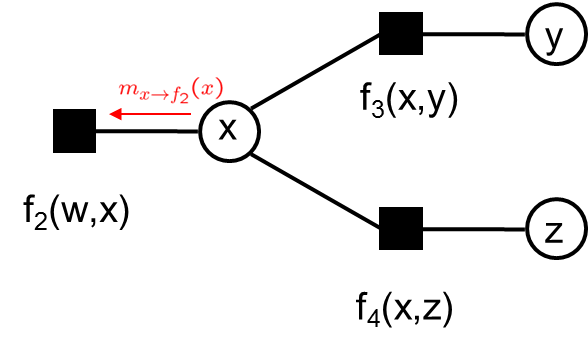
\includegraphics[width=0.4\textwidth]{ExampleMessages3}
}
\[
\Red{m_{x\rightarrow f_2}(x)} = \sum_y\sum_z f_3(x,y)f_4(x,z)
\]

\phantom{.}
\hfill
\phantom{.}

\end{frame}


\begin{frame}
\frametitle{Messages: from variables to factors (2)}

\centerline{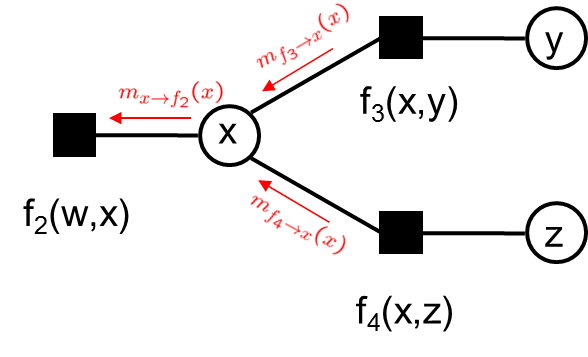
\includegraphics[width=0.4\textwidth]{ExampleMessages4}}

\begin{eqnarray*}
\Red{m_{x\rightarrow f_2}(x)} &=& \sum_y\sum_z f_3(x,y)f_4(x,z) \\
&= &
\underbrace{\Big[\!\sum_y f_3(x,y)\!\Big]}_{\Red{m_{f_3\rightarrow x}(x)}}
\cdot
\underbrace{\Big[\!\sum_z f_4(x,z)\!\Big]}_{\Red{m_{f_4\rightarrow x}(x)}}
\end{eqnarray*}

\begin{itemize}
\item Variables pass on the product of all incoming messages.
\end{itemize}

\end{frame}


\begin{frame}
\frametitle{Factor graph marginalisation: summary}

\centerline{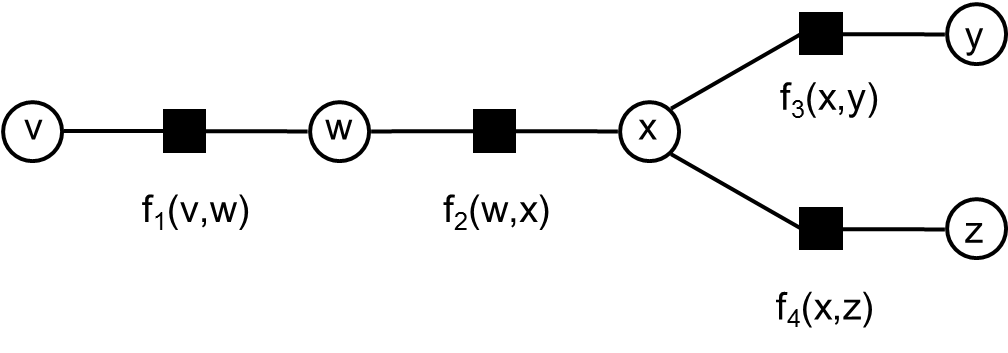
\includegraphics[width=0.6\textwidth]{ExampleFactorGraph1}
}
\vspace{-4mm}
\begin{align*}
p(w) &= \sum_v\sum_x\sum_y\sum_z f_1(v,w)f_2(w,x)f_3(x,y)f_4(x,z)\\
&= 
\underbrace{\Big[\!\sum_v f_1(v,w)\!\Big]}_{\Red{m_{f_1\rightarrow w}(w)}}\cdot
\underbrace{\Big[\!
\sum_x f_2(w,x) \cdot
\underbrace{\Big[\!
\underbrace{\Big[\!\sum_y f_3(x,y)\!\Big]}_{\Red{m_{f_3\rightarrow x}(x)}}
\cdot
\underbrace{\Big[\!\sum_z f_4(x,z)\!\Big]}_{\Red{m_{f_4\rightarrow x}(x)}}
\!\Big]}_{\Red{m_{x\rightarrow f_2}(x)}}
\!\Big]}_{\Red{m_{f_2\rightarrow w}(w)}}
\end{align*}
%
\vspace{-3mm}
\begin{itemize}
\item The complexity is reduced from ${\cal O}(K^5)$ (naïve implementation) to ${\cal O}(K^2)$.
\end{itemize}

\end{frame}


\begin{frame}
\frametitle{The sum-product algorithm}

In summary, message passing involved three update equations:
\begin{itemize}
\item Marginals are the product of all incoming messages from neighbour factors
\[
p(t) = \prod_{f\in F_t}m_{f\rightarrow t}(t)
\]
\item Messages from factors sum out all variables except the receiving one
\[
m_{f\rightarrow {t_1}}(t_1) = \sum_{t_2}\sum_{t_3}\ldots\sum_{t_n}f(t_1,t_2,\ldots,t_n)
\prod_{i \neq 1} m_{t_i\rightarrow f}(t_i)
\]
\item Messages from variables are the product of all incoming messages 
except the message from the receiving factor
\[
m_{t\rightarrow f}(t) = \prod_{f_j\in F_t\backslash \{f\}}
m_{f_j\rightarrow t}(t) = \frac{p(t)}{m_{f\rightarrow t}(t)}
\]
\end{itemize}
Messages are results of \Blue{partial computations}. Computations are \Blue{localised}.

\end{frame}

\end{document}
